% omega.tex --
%%%%%%%%%%%%%%%%%%%%%%%%%%%%%%%%%%%%%%%%%%%%%%%%%%%%%%%%%%%%%%%%%%%%%%%%
\NeedsTeXFormat{LaTeX2e}
\RequirePackage{ifpdf}
\ifpdf
  \documentclass[a4paper,notitlepage,chapters]{flex}
  \usepackage{type1cm}
  \usepackage[pdftex,colorlinks]{hyperref}
  \usepackage[pdftex]{graphicx,feynmp,emp}
  \DeclareGraphicsRule{*}{mps}{*}{}
\else
  \documentclass[a4paper,notitlepage,chapters]{flex}
  \usepackage[T1]{fontenc}
  % \usepackage[hypertex]{hyperref}
  \usepackage{graphicx,feynmp,emp}
\fi
\usepackage{verbatim,array,amsmath,amssymb}
\usepackage{url,thophys,thohacks}
\setlength{\unitlength}{1mm}
\empaddtoTeX{\usepackage{amsmath,amssymb}}
\empaddtoTeX{\usepackage{thophys,thohacks}}
\empaddtoprelude{input graph;}
\empaddtoprelude{input boxes;}
%%%%%%%%%%%%%%%%%%%%%%%%%%%%%%%%%%%%%%%%%%%%%%%%%%%%%%%%%%%%%%%%%%%%%%%%
%%% This should be part of flex.cls and/or thopp.sty
\makeatletter
  \@ifundefined{frontmatter}%
    {\def\frontmatter{\pagenumbering{roman}}%
     \def\mainmatter{\cleardoublepage\pagenumbering{arabic}}}
    {}
\makeatother
%%%%%%%%%%%%%%%%%%%%%%%%%%%%%%%%%%%%%%%%%%%%%%%%%%%%%%%%%%%%%%%%%%%%%%%%
%%% \makeatletter
%%% %%% Italic figure captions to separate them visually from the text
%%% %%% (this should be supported by flex.cls):
%%% \makeatletter
%%%   \@secpenalty=-1000
%%%   \def\fps@figure{t}
%%%   \def\fps@table{b}
%%%   \long\def\@makecaption#1#2{%
%%%     \vskip\abovecaptionskip
%%%     \sbox\@tempboxa{#1: \textit{#2}}%
%%%     \ifdim\wd\@tempboxa>\hsize
%%%       #1: \textit{#2}\par
%%%     \else
%%%       \global\@minipagefalse
%%%       \hb@xt@\hsize{\hfil\box\@tempboxa\hfil}%
%%%     \fi
%%%     \vskip\belowcaptionskip}
%%% \makeatother
\widowpenalty=4000
\clubpenalty=4000
\displaywidowpenalty=4000
%%% \pagestyle{headings}
%%%%%%%%%%%%%%%%%%%%%%%%%%%%%%%%%%%%%%%%%%%%%%%%%%%%%%%%%%%%%%%%%%%%%%%%
\allowdisplaybreaks
\renewcommand{\topfraction}{0.8}
\renewcommand{\bottomfraction}{0.8}
\renewcommand{\textfraction}{0.2}
\setlength{\abovecaptionskip}{.5\baselineskip}
\setlength{\belowcaptionskip}{\baselineskip}
%%%%%%%%%%%%%%%%%%%%%%%%%%%%%%%%%%%%%%%%%%%%%%%%%%%%%%%%%%%%%%%%%%%%%%%%
%%% allow VERY overfull hboxes
\setlength{\hfuzz}{5cm}
%%%%%%%%%%%%%%%%%%%%%%%%%%%%%%%%%%%%%%%%%%%%%%%%%%%%%%%%%%%%%%%%%%%%%%%%
\usepackage{noweb}
%%% \usepackage{nocondmac}
\setlength{\nwmarginglue}{1em}
\noweboptions{smallcode,noidentxref}%%%{webnumbering}
%%% Saving paper:
\def\nwendcode{\endtrivlist\endgroup}
\nwcodepenalty=0
\let\nwdocspar\relax
%%%%%%%%%%%%%%%%%%%%%%%%%%%%%%%%%%%%%%%%%%%%%%%%%%%%%%%%%%%%%%%%%%%%%%%%
\newcommand{\ttfilename}[1]{\texttt{\detokenize{#1}}}
\usepackage[noweb,bypages]{ocamlweb}
\empaddtoTeX{\usepackage[noweb,bypages]{ocamlweb}}
\renewcommand{\ocwinterface}[1]{\section{Interface of \ocwupperid{#1}}}
\renewcommand{\ocwmodule}[1]{\section{Implementation of \ocwupperid{#1}}}
\renewcommand{\ocwinterfacepart}{\relax}
\renewcommand{\ocwcodepart}{\relax}
\renewcommand{\ocwbeginindex}{\begin{theindex}}
\newcommand{\thocwmodulesection}[1]{\subsection{#1}}
\newcommand{\thocwmodulesubsection}[1]{\subsubsection{#1}}
\newcommand{\thocwmoduleparagraph}[1]{\paragraph{#1}}
\renewcommand{\ocwindent}[1]{\noindent\ignorespaces}
\renewcommand{\ocwbegincode}{\renewcommand{\ocwindent}[1]{\noindent\kern##1}}
\renewcommand{\ocwendcode}{\renewcommand{\ocwindent}[1]{\noindent\ignorespaces}}
\renewcommand{\ocweol}{\setlength\parskip{0pt}\par}
\makeatletter
\renewcommand{\@oddfoot}{\reset@font\hfil\thepage\hfil}
\let\@evenfoot\@oddfoot
\def\@evenhead{\leftmark{} \hrulefill}%
\def\@oddhead{\hrulefill{} \rightmark}%
\let\@mkboth\markboth
\renewcommand{\chaptermark}[1]{\markboth{\hfil}{\hfil}}%
\renewcommand{\sectionmark}[1]{\markboth{#1}{#1}}
\renewcommand{\chapter}{%
  \clearpage\global\@topnum\z@\@afterindentfalse
  \secdef\@chapter\@schapter}
\makeatother
\newcommand{\signature}[1]{%
  \InputIfFileExists{#1.interface}{}%
    {\begin{dubious}\textit{Interface \ttfilename{#1.mli} unavailable!}\end{dubious}}}
\newcommand{\application}[1]{%
  \InputIfFileExists{#1.implementation}{}%
    {\begin{dubious}\textit{Application \ttfilename{#1.ml} unavailable!}\end{dubious}}}
\newcommand{\module}[1]{%
  \label{mod:#1}%
  \InputIfFileExists{#1.interface}{}%
    {\begin{dubious}\textit{Interface \ttfilename{#1.mli} unavailable!}\end{dubious}}%
  \InputIfFileExists{#1.implementation}{}%
    {\begin{dubious}\textit{Implementation \ttfilename{#1.ml} unavailable!}\end{dubious}}}
\newcommand{\lexer}[1]{\application{#1_lexer}}
\renewcommand{\ocwlexmodule}[1]{\relax}
\newcommand{\parser}[1]{\application{#1_parser}}
\renewcommand{\ocwyaccmodule}[1]{\relax}
\newcommand{\thocwincludegraphics}[2]{\includegraphics[#1]{#2}}
\ifpdf
  \newcommand{\thocwdefref}[1]{\textbf{\pageref{#1}}}%
  \newcommand{\thocwuseref}[1]{\textrm{\pageref{#1}}}%
  \renewcommand{\ocwrefindexentry}[5]%
    {\item #1,\quad\let\ref\thocwdefref{#4}, used: \let\ref\thocwuseref{#5}}
\fi
\newcommand{\thocwmakebox}[4]{\makebox(#1,#2)[#3]{#4}}
%%%%%%%%%%%%%%%%%%%%%%%%%%%%%%%%%%%%%%%%%%%%%%%%%%%%%%%%%%%%%%%%%%%%%%%%
\newenvironment{modules}[1]%
 {\begin{list}{}%
   {\setlength{\leftmargin}{3em}%
    \setlength{\rightmargin}{2em}%
    \setlength{\itemindent}{-1em}%
    \setlength{\listparindent}{0pt}%
    %%%\setlength{\itemsep}{0pt}%
    \settowidth{\labelwidth}{\textbf{\ocwupperid{#1}:}}%
    \renewcommand{\makelabel}[1]{\ocwupperid{##1:}}}}%
 {\end{list}}
\newenvironment{JR}%
  {\begin{dubious}\textit{JR sez' (regarding the Majorana Feynman rules):}}
  {\textit{(JR's probably right, but I need to check myself \ldots)}
   \end{dubious}}
  
%%%%%%%%%%%%%%%%%%%%%%%%%%%%%%%%%%%%%%%%%%%%%%%%%%%%%%%%%%%%%%%%%%%%%%%%
\DeclareMathOperator{\tr}{tr}
\newcommand{\dd}{\mathrm{d}}
\newcommand{\ii}{\mathrm{i}}
\newcommand{\ee}{\mathrm{e}}
\renewcommand{\Re}{\text{Re}}
\renewcommand{\Im}{\text{Im}}
\newcommand{\ketbra}[2]{\ket{#1}\!\bra{#2}}
\newcommand{\Ketbra}[2]{\Ket{#1}\!\Bra{#2}}

%%%%%%%%%%%%%%%%%%%%%%%%%%%%%%%%%%%%%%%%%%%%%%%%%%%%%%%%%%%%%%%%%%%%%%%%
\makeindex
\begin{document}
\begin{fmffile}{\jobname pics}
\fmfset{arrow_ang}{10}
\fmfset{curly_len}{2mm}
\fmfset{wiggly_len}{3mm}
%%%%%%%%%%%%%%%%%%%%%%%%%%%%%%%%%%%%%%%%%%%%%%%%%%%%%%%%%%%%%%%%%%%%%%%%
\fmfcmd{%
  numeric joindiameter;
  joindiameter := 7thick;}
\fmfcmd{%
  vardef sideways_at (expr d, p, frac) =
    save len; len = length p;
    (point frac*len of p) shifted ((d,0) rotated (90 + angle direction frac*len of p))
  enddef;
  secondarydef p sideways d =
    for frac = 0 step 0.01 until 0.99:
      sideways_at (d, p, frac) ..
    endfor
    sideways_at (d, p, 1)
  enddef;
  secondarydef p choptail d =
   subpath (ypart (fullcircle scaled d shifted (point 0 of p) intersectiontimes p), infinity) of p
  enddef;
  secondarydef p choptip d =
   reverse ((reverse p) choptail d)
  enddef;
  secondarydef p pointtail d =
    fullcircle scaled d shifted (point 0 of p) intersectionpoint p
  enddef;
  secondarydef p pointtip d =
    (reverse p) pointtail d
  enddef;
  secondarydef pa join pb =
    pa choptip joindiameter .. pb choptail joindiameter
  enddef;
  vardef cyclejoin (expr p) =
    subpath (0.5*length p, infinity) of p join subpath (0, 0.5*length p) of p .. cycle
  enddef;}
%%%%%%%%%%%%%%%%%%%%%%%%%%%%%%%%%%%%%%%%%%%%%%%%%%%%%%%%%%%%%%%%%%%%%%%%
\fmfcmd{%
  style_def double_line_arrow expr p =
    save pi, po; 
    path pi, po;
    pi = reverse (p sideways thick);
    po = p sideways -thick;
    cdraw pi;
    cdraw po;
    cfill (arrow pi);
    cfill (arrow po);
  enddef;}
\fmfcmd{%
  style_def double_line_arrow_beg expr p =
    save pi, po, pc; 
    path pi, po, pc;
    pc = p choptail 7thick;
    pi = reverse (pc sideways thick);
    po = pc sideways -thick;
    cdraw pi .. p pointtail 5thick .. po;
    cfill (arrow pi);
    cfill (arrow po);
  enddef;}
\fmfcmd{%
  style_def double_line_arrow_end expr p =
    save pi, po, pc; 
    path pi, po, pc;
    pc = p choptip 7thick;
    pi = reverse (pc sideways thick);
    po = pc sideways -thick;
    cdraw po .. p pointtip 5thick .. pi;
    cfill (arrow pi);
    cfill (arrow po);
  enddef;}
\fmfcmd{%
  style_def double_line_arrow_both expr p =
    save pi, po, pc; 
    path pi, po, pc;
    pc = p choptip 7thick choptail 7thick;
    pi = reverse (pc sideways thick);
    po = pc sideways -thick;
    cdraw po .. p pointtip 5thick .. pi .. p pointtail 5thick .. cycle;
    cfill (arrow pi);
    cfill (arrow po);
  enddef;}
%%%%%%%%%%%%%%%%%%%%%%%%%%%%%%%%%%%%%%%%%%%%%%%%%%%%%%%%%%%%%%%%%%%%%%%%
\fmfcmd{vardef middir (expr p, ang) =
    dir (angle direction length(p)/2 of p + ang)
  enddef;}
\fmfcmd{style_def arrow_left expr p =
    shrink (.7);
      cfill (arrow p shifted (4thick * middir (p, 90)));
    endshrink
  enddef;}
\fmfcmd{style_def arrow_right expr p =
    shrink (.7);
      cfill (arrow p shifted (4thick * middir (p, -90)));
    endshrink
  enddef;}
\fmfcmd{style_def warrow_left expr p =
    shrink (.7);
      cfill (arrow p shifted (8thick * middir (p, 90)));
    endshrink
  enddef;}
\fmfcmd{style_def warrow_right expr p =
    shrink (.7);
      cfill (arrow p shifted (8thick * middir (p, -90)));
    endshrink
  enddef;}
%%%%%%%%%%%%%%%%%%%%%%%%%%%%%%%%%%%%%%%%%%%%%%%%%%%%%%%%%%%%%%%%%%%%%%%%
\newcommand{\threeexternal}[3]{%
  \fmfsurround{d1,e1,d2,e2,d3,e3}%
  \fmfv{label=$#1$,label.ang=0}{e1}%
  \fmfv{label=$#2$,label.ang=180}{e2}%
  \fmfv{label=$#3$,label.ang=0}{e3}}
\newcommand{\Threeexternal}[3]{%
  \fmfsurround{d1,e1,d3,e3,d2,e2}%
  \fmfv{label=$#1$,label.ang=0}{e1}%
  \fmfv{label=$#2$,label.ang=0}{e2}%
  \fmfv{label=$#3$,label.ang=180}{e3}}
\newcommand{\Fourexternal}[4]{%
  \fmfsurround{d2,e2,d1,e1,d4,e4,d3,e3}%
  \fmfv{label=$#1$,label.ang=180}{e1}%
  \fmfv{label=$#2$,label.ang=0}{e2}%
  \fmfv{label=$#3$,label.ang=0}{e3}%
  \fmfv{label=$#4$,label.ang=180}{e4}}
\newcommand{\Fiveexternal}[5]{%
  \fmfsurround{d2,e2,d1,e1,d5,e5,d4,e4,d3,e3}%
  \fmfv{label=$#1$,label.ang=180}{e1}%
  \fmfv{label=$#2$,label.ang=0}{e2}%
  \fmfv{label=$#3$,label.ang=0}{e3}%
  \fmfv{label=$#4$,label.ang=0}{e4}%
  \fmfv{label=$#5$,label.ang=180}{e5}}
\newcommand{\twoincoming}{%
    \fmfdot{v}%
    \fmffreeze%
    \fmf{warrow_right}{e1,v}%
    \fmf{warrow_right}{e2,v}%
    \fmf{warrow_right}{v,e3}}
\newcommand{\threeincoming}{%
    \fmfdot{v}%
    \fmffreeze%
    \fmf{warrow_right}{e1,v}%
    \fmf{warrow_right}{e2,v}%
    \fmf{warrow_right}{e3,v}}
\newcommand{\threeoutgoing}{%
    \fmfdot{v}%
    \fmffreeze%
    \fmf{warrow_right}{v,e1}%
    \fmf{warrow_right}{v,e2}%
    \fmf{warrow_right}{v,e3}}
\newcommand{\fouroutgoing}{%
    \threeoutgoing%
    \fmf{warrow_right}{v,e4}}
\newcommand{\fiveoutgoing}{%
    \fouroutgoing%
    \fmf{warrow_right}{v,e5}}
\newcommand{\setupthreegluons}{%
  \fmftop{g3}
  \fmfbottom{g1,g2}
  \fmf{phantom}{v,g1}
  \fmf{phantom}{v,g2}
  \fmf{phantom}{v,g3}
  \fmffreeze
  \fmfipair{v,g[],a[],b[]}
  \fmfiset{g1}{vloc (__g1)}
  \fmfiset{g2}{vloc (__g2)}
  \fmfiset{g3}{vloc (__g3)}
  \fmfiset{v}{vloc (__v)}
  \fmfiset{a1}{g1 shifted (-3thin,0)}
  \fmfiset{b1}{g1 shifted (+1thin,-2thin)}
  \fmfiset{a2}{g2 shifted (0,-3thin)}
  \fmfiset{b2}{g2 shifted (0,+3thin)}
  \fmfiset{a3}{g3 shifted (+1thin,+2thin)}
  \fmfiset{b3}{g3 shifted (-3thin,0)}}
\begin{empfile}
%%%%%%%%%%%%%%%%%%%%%%%%%%%%%%%%%%%%%%%%%%%%%%%%%%%%%%%%%%%%%%%%%%%%%%%%
\frontmatter
\title{
  O'Mega:\\
  Optimal~Monte-Carlo\\
  Event~Generation~Amplitudes}
\author{%
  Thorsten Ohl\thanks{%
    \texttt{ohl@physik.uni-wuerzburg.de},
    \texttt{http://physik.uni-wuerzburg.de/ohl}}\\
  \hfil\\
    Institut f\"ur Theoretische~Physik und Astrophysik\\
    Julius-Maximilians-Universit\"at~W\"urzburg\\
    Emil-Hilb-Weg 22, 97074~W\"urzburg, Germany\\
  \hfil\\
  J\"urgen Reuter\thanks{\texttt{juergen.reuter@desy.de}}\\
  \hfil\\
    DESY Theory Group,
    Notkestr. 85, 22603 Hamburg, Germany\\
  \hfil\\
  Wolfgang Kilian${}^{c,}$\thanks{\texttt{kilian@physik.uni-siegen.de}}\\
  \hfil\\
    Theoretische Physik 1\\
    Universit\"at Siegen\\
    Walter-Flex-Str.~3, 57068 Siegen, Germany\\ 
  \hfil\\
  with contributions from 
  Christian
  Speckner${}^{d,}$\thanks{\texttt{cnspeckn@googlemail.com}}\\
  as well as 
  Christian Schwinn et al.}
\date{\textbf{unpublished draft, printed \timestamp}}
\maketitle
\begin{abstract}
  \ldots
\end{abstract}
%%%%%%%%%%%%%%%%%%%%%%%%%%%%%%%%%%%%%%%%%%%%%%%%%%%%%%%%%%%%%%%%%%%%%%%%
\newpage
\begin{quote}
  Copyright \textcopyright~1999-2013 by
  \begin{itemize}
    \item Wolfgang~Kilian ~\texttt{<kilian@hep.physik.uni-siegen.de>}
    \item Thorsten~Ohl~\texttt{<ohl@physik.uni-wuerzburg.de>}
    \item J\"urgen~Reuter~\texttt{<juergen.reuter@desy.de>}
  \end{itemize}
\end{quote}
\begin{quote}
  WHIZARD is free software; you can redistribute it and/or modify it under
  the terms of the GNU General Public License as published by the Free
  Software Foundation; either version 2, or (at your option) any later
  version.
\end{quote}
\begin{quote}
  WHIZARD is distributed in the hope that it will be useful, but
  \emph{without any warranty}; without even the implied warranty of
  \emph{merchantability} or \emph{fitness for a particular purpose}.
  See the GNU General Public License for more details.
\end{quote}
\begin{quote}
  You should have received a copy of the GNU General Public License
  along with this program; if not, write to the Free Software
  Foundation, Inc., 675 Mass Ave, Cambridge, MA 02139, USA.
\end{quote}
\setcounter{tocdepth}{2}
\tableofcontents
\mainmatter

%%%%%%%%%%%%%%%%%%%%%%%%%%%%%%%%%%%%%%%%%%%%%%%%%%%%%%%%%%%%%%%%%%%%%%%%
\chapter{Introduction}
\label{sec:intro}

%%%%%%%%%%%%%%%%%%%%%%%%%%%%%%%%%%%%%%%%%%%%%%%%%%%%%%%%%%%%%%%%%%%%%%%%
\section{Complexity}
\label{sec:complexity}

\begin{table}
  \begin{center}
     \begin{tabular}{r|r|r}
       $n$ & $P(n)$& $F(n)$ \\\hline
         4 &     3 & 3      \\
         5 &    10 & 15     \\
         6 &    25 & 105    \\
         7 &    56 & 945    \\
         8 &   119 & 10395  \\
         9 &   246 & 135135 \\
        10 &   501 & 2027025 \\
        11 &  1012 & 34459425 \\
        12 &  2035 & 654729075 \\
        13 &  4082 & 13749310575 \\
        14 &  8177 & 316234143225 \\
        15 & 16368 & 7905853580625 \\
        16 & 32751 & 213458046676875
     \end{tabular}
  \end{center}
  \caption{\label{tab:P(n),F(n)}
    The number of $\phi^3$ Feynman diagrams~$F(n)$ and independent
    poles~$P(n)$.}
\end{table}
There are
\begin{equation}
  P(n) = \frac{2^n-2}{2} - n = 2^{n-1} - n - 1
\end{equation}
independent internal momenta in a $n$-particle scattering
amplitude~\cite{ALPHA:1997}.  This grows much slower than the
number
\begin{equation}
  F(n) = (2n-5)!! = (2n-5)\cdot(2n-7)\cdot\ldots\cdot3\cdot1
\end{equation}
of tree Feynman diagrams in vanilla $\phi^3$ (see
table~\ref{tab:P(n),F(n)}).  There are no known corresponding
expressions for theories with more than one particle type.  However,
empirical evidence from numerical studies~\cite{ALPHA:1997,HELAC:2000}
as well as explicit counting results from O'Mega suggest
\begin{equation}
  P^*(n) \propto 10^{n/2}
\end{equation}
while he factorial growth of the number of Feynman diagrams remains
unchecked, of course.

The number of independent momenta in an amplitude is a better measure
for the complexity of the amplitude than the number of Feynman
diagrams, since there can be substantial cancellations among the
latter.  Therefore it should be possible to express the scattering
amplitude more compactly than by a sum over Feynman diagrams.

%%%%%%%%%%%%%%%%%%%%%%%%%%%%%%%%%%%%%%%%%%%%%%%%%%%%%%%%%%%%%%%%%%%%%%%%
\section{Ancestors}
\label{sec:ancestors}

Some of the ideas that O'Mega is based on can be traced back to
HELAS~\cite{HELAS}.  HELAS builts Feynman amplitudes by recursively
forming off-shell `wave functions' from joining external lines with
other external lines or off-shell `wave functions'.

The program Madgraph~\cite{MADGRAPH:1994} automatically generates
Feynman diagrams and writes a Fortran program corresponding to their
sum.  The amplitudes are calculated by calls to HELAS~\cite{HELAS}.
Madgraph uses one straightforward optimization: no statement is
written more than once.  Since each statement corresponds to a
collection of trees, this optimization is very effective for up to
four particles in the final state.  However, since the amplitudes are
given as a sum of Feynman diagrams, this optimization can, by design,
\emph{not} remove the factorial growth and is substantially weaker
than the algorithms of~\cite{ALPHA:1997,HELAC:2000} and the algorithm
of O'Mega for more particles in the final state.

Then ALPHA~\cite{ALPHA:1997} (see also the slightly modified
variant~\cite{HELAC:2000}) provided a numerical algorithm for
calculating scattering amplitudes and it could be shown empirically,
that the calculational costs are rising with a power instead of
factorially.

%%%%%%%%%%%%%%%%%%%%%%%%%%%%%%%%%%%%%%%%%%%%%%%%%%%%%%%%%%%%%%%%%%%%%%%%
\section{Architecture}
\label{sec:architecture}

\begin{figure}
  \begin{center}
    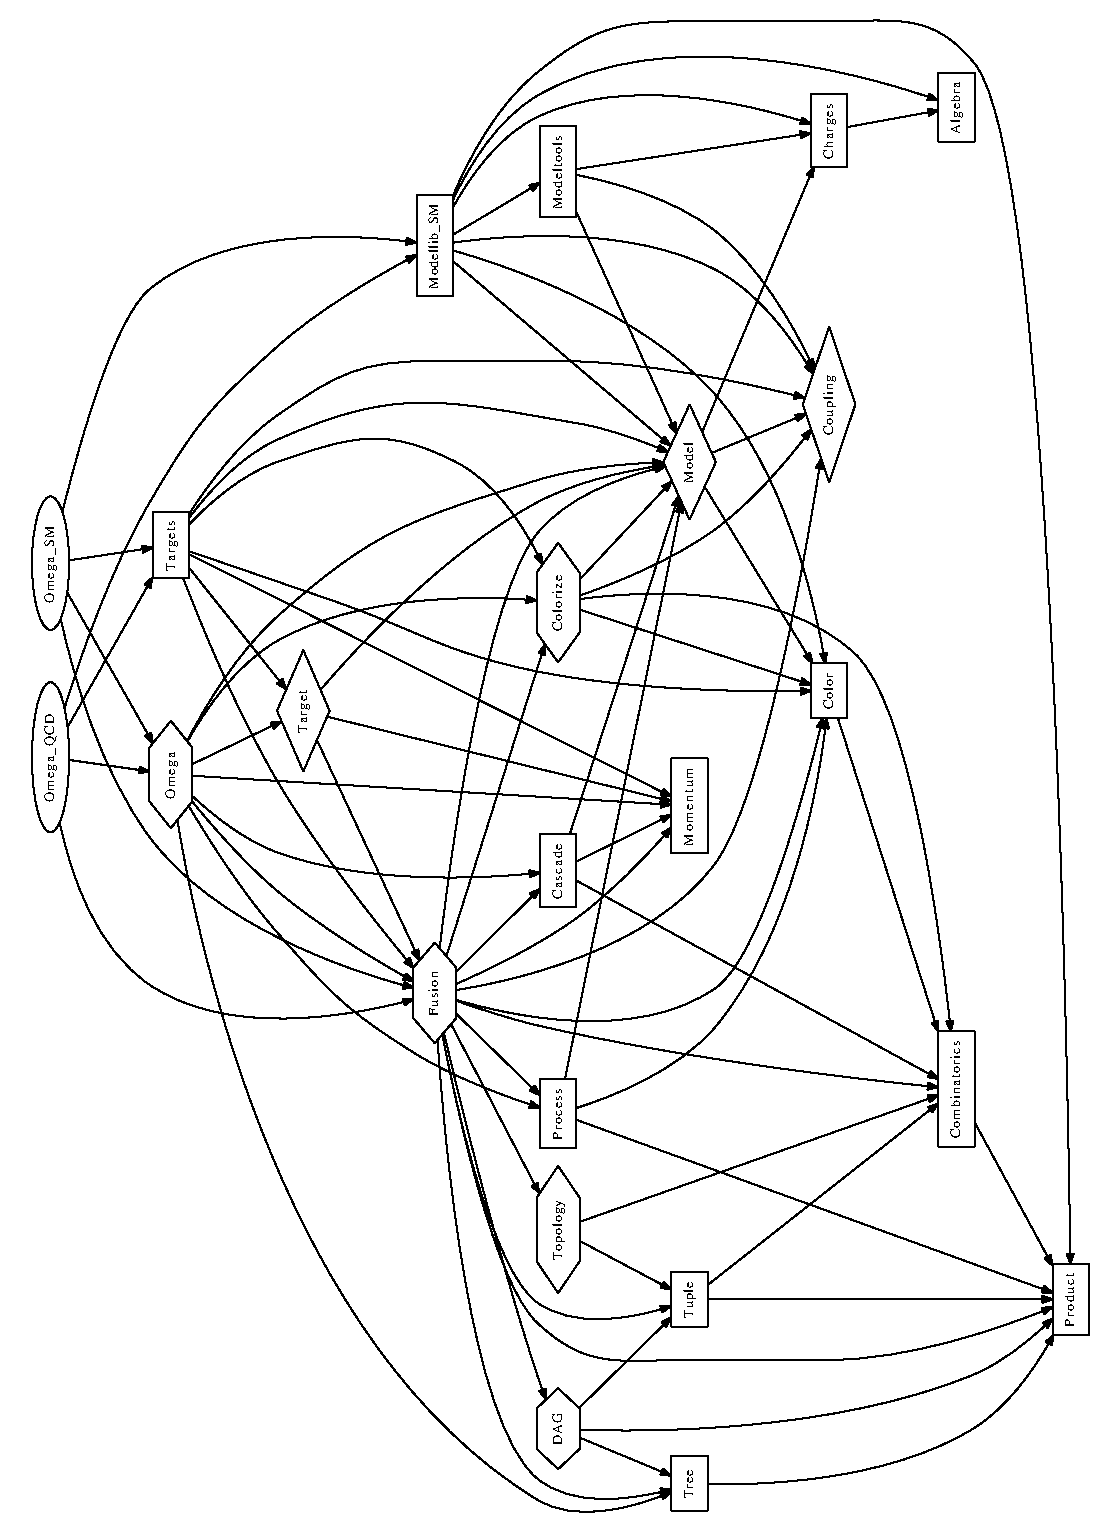
\includegraphics[width=\textwidth]{modules}
    %includegraphics[height=.8\textheight]{modules}
  \end{center}
  \caption{\label{fig:modules}%
    Module dependencies in O'Mega.}
    %% The diamond shaped nodes are abstract signatures defininng functor
    %% domains and co-domains. The rectangular boxes are modules and
    %% functors and oval boxes are examples for applications.
\end{figure}

\subsection{General purpose libraries}
Functions that are not specific to O'Mega and could be part of the
O'Caml standard library
\begin{modules}{}
  \item[ThoList] (mostly) simple convenience functions for lists that
    are missing from the standard library module \ocwupperid{List}
    (section~\ref{sec:tholist}, p.~\pageref{sec:tholist})
  \item[Product] effcient tensor products for lists and sets
    (section~\ref{sec:product}, p.~\pageref{sec:product})
  \item[Combinatorics] combinatorical formulae, sets of subsets, etc. 
    (section~\ref{sec:combinatorics}, p.~\pageref{sec:combinatorics})
\end{modules}

\subsection{O'Mega}
The non-trivial algorithms that constitute O'Mega:
\begin{modules}{}
  \item[DAG] Directed Acyclical Graphs
    (section~\ref{sec:DAG}, p.~\pageref{sec:DAG})
  \item[Topology] unusual enumerations of unflavored tree diagrams
    (section~\ref{sec:topology}, p.~\pageref{sec:topology})
  \item[Momentum] finite sums of external momenta
    (section~\ref{sec:momentum}, p.~\pageref{sec:momentum})
  \item[Fusion] off shell wave functions
    (section~\ref{sec:fusion}, p.~\pageref{sec:fusion})
  \item[Omega] functor constructing an application from a model and a
    target
    (section~\ref{sec:omega}, p.~\pageref{sec:omega})
\end{modules}

\subsection{Abstract interfaces}
The domains and co-domains of functors
(section~\ref{sec:coupling}, p.~\pageref{sec:coupling})
\begin{modules}{}
  \item[Coupling] all possible couplings (not comprensive yet)
  \item[Model] physical models
  \item[Target] target programming languages
\end{modules}

\subsection{Models}
(section~\ref{sec:models}, p.~\pageref{sec:models})
\begin{modules}{}
  \item[Modellib_SM.QED] Quantum Electrodynamics
  \item[Modellib_SM.QCD] Quantum Chromodynamics (not complete yet)
  \item[Modellib_SM.SM] Minimal Standard Model (not complete yet)
\end{modules}
etc.

\subsection{Targets}
Any programming language that supports arithmetic and a textual
representation of programs can be targeted by O'Caml.  The
implementations translate the abstract expressions derived by
\ocwupperid{Fusion} to expressions in the target
(section~\ref{sec:targets}, p.~\pageref{sec:targets}).
\begin{modules}{}
  \item[Targets.Fortran] Fortran95 language implementation, calling
    subroutines
\end{modules}
Other targets could come in the future: \texttt{C}, \texttt{C++},
O'Caml itself, symbolic manipulation languages, etc.

\subsection{Applications}
(section~\ref{sec:omega}, p.~\pageref{sec:omega})

%%%%%%%%%%%%%%%%%%%%%%%%%%%%%%%%%%%%%%%%%%%%%%%%%%%%%%%%%%%%%%%%%%%%%%%%
\section{The Big To Do Lists}
\label{sec:TODO}

%%%%%%%%%%%%%%%%%%%%%%%%%%%%%%%%%%%%%%%%%%%%%%%%%%%%%%%%%%%%%%%%%%%%%%%%
\subsection{Required}
All features required for leading order physics applications are in place.

%%%%%%%%%%%%%%%%%%%%%%%%%%%%%%%%%%%%%%%%%%%%%%%%%%%%%%%%%%%%%%%%%%%%%%%%
\subsection{Useful}
\begin{enumerate}
  \item select allowed helicity combinations for massless fermions
  \item Weyl-Van der Waerden spinors
  \item speed up helicity sums by using discrete symmetries
  \item general triple and quartic vector couplings
  \item diagnostics: count corresponding Feynman diagrams 
    more efficiently for more than ten external lines
  \item recognize potential cascade decays ($\tau$, $b$, etc.)
    \begin{itemize}
      \item warn the user to add additional
      \item kill fusions (at runtime), that contribute to a cascade
    \end{itemize}
  \item complete standard model in $R_\xi$-gauge
  \item groves (the simple method of cloned generations works)
\end{enumerate}

%%%%%%%%%%%%%%%%%%%%%%%%%%%%%%%%%%%%%%%%%%%%%%%%%%%%%%%%%%%%%%%%%%%%%%%%
\subsection{Future Features}
\begin{enumerate}
  \item investigate if unpolarized squared matrix elements can be
    calculated faster as traces of densitiy matrices.  Unfortunately,
    the answer apears to be \emph{no} for fermions and \emph{up to a
    constant factor} for massive vectors.  Since the number of fusions
    in the amplitude grows like~$10^{n/2}$, the number of fusions in
    the squared matrix element grows like~$10^n$.  On the other hand,
    there are $2^{\#\text{fermions}+\#\text{massless vectors}}
    \cdot3^{\#\text{massive vectors}}$ terms in the helicity sum, which
    grows \emph{slower} than~$10^{n/2}$.  The constant factor is
    probably also not favorable.
    However, there will certainly be asymptotic gains for sums over
    gauge (and other) multiplets, like color sums.
  \item compile Feynman rules from Lagrangians
  \item evaluate amplitues in O'Caml by compiling it to three address
    code for a virtual machine
    \begin{flushleft}
      \ocwkw{type}~$\ocwlowerid{mem}~=~\ocwlowerid{scalar}~$\ocwbt{array}~$%
        \times{}~\ocwlowerid{spinor}~$\ocwbt{array}~$%
        \times{}~\ocwlowerid{spinor}~$\ocwbt{array}~$%
        \times{}~\ocwlowerid{vector}~$\ocwbt{array}\\
      \ocwkw{type}~$\ocwlowerid{instr}~=$\\
      \qquad|~$\ocwupperid{VSS}~$\ocwkw{of}~\ocwbt{int}~$%
        \times{}~$\ocwbt{int}~$\times{}~$\ocwbt{int}\\
      \qquad|~$\ocwupperid{SVS}~$\ocwkw{of}~\ocwbt{int}~$%
        \times{}~$\ocwbt{int}~$\times{}~$\ocwbt{int}\\
      \qquad|~$\ocwupperid{AVA}~$\ocwkw{of}~\ocwbt{int}~$%
        \times{}~$\ocwbt{int}~$\times{}~$\ocwbt{int}\\
      \qquad\ldots
    \end{flushleft}
    this could be as fast as~\cite{ALPHA:1997} or~\cite{HELAC:2000}.
  \item a virtual machine will be useful for for other target as
    well, because native code appears to become to large for most
    compilers for more than ten external particles.  Bytecode might
    even be faster due to improved cache locality.
  \item use the virtual machine in O'Giga
\end{enumerate}

%%%%%%%%%%%%%%%%%%%%%%%%%%%%%%%%%%%%%%%%%%%%%%%%%%%%%%%%%%%%%%%%%%%%%%%%
\subsection{Science Fiction}
\begin{enumerate}
  \item numerical and symbolical loop calculations with
    \textsc{O'Tera: O'Mega Tool for Evaluating Renormalized Amplitudes}
\end{enumerate}

%%%%%%%%%%%%%%%%%%%%%%%%%%%%%%%%%%%%%%%%%%%%%%%%%%%%%%%%%%%%%%%%%%%%%%%%
\chapter{Tuples and Polytuples}
\label{sec:tuple}
\module{tuple}

%%%%%%%%%%%%%%%%%%%%%%%%%%%%%%%%%%%%%%%%%%%%%%%%%%%%%%%%%%%%%%%%%%%%%%%%
\chapter{Topologies}
\label{sec:topology}
\module{topology}

%%%%%%%%%%%%%%%%%%%%%%%%%%%%%%%%%%%%%%%%%%%%%%%%%%%%%%%%%%%%%%%%%%%%%%%%
\chapter{Directed Acyclical Graphs}
\label{sec:DAG}
\module{dAG}

%%%%%%%%%%%%%%%%%%%%%%%%%%%%%%%%%%%%%%%%%%%%%%%%%%%%%%%%%%%%%%%%%%%%%%%%
\chapter{Momenta}
\label{sec:momentum}
\module{momentum}

%%%%%%%%%%%%%%%%%%%%%%%%%%%%%%%%%%%%%%%%%%%%%%%%%%%%%%%%%%%%%%%%%%%%%%%%
\chapter{Cascades}
\label{sec:cascades}
\module{cascade_syntax}
\section{Lexer}
\lexer{cascade}
\section{Parser}
\parser{cascade}
\module{cascade}

%%%%%%%%%%%%%%%%%%%%%%%%%%%%%%%%%%%%%%%%%%%%%%%%%%%%%%%%%%%%%%%%%%%%%%%%
\chapter{Color}
\label{sec:color}
\module{color}

%%%%%%%%%%%%%%%%%%%%%%%%%%%%%%%%%%%%%%%%%%%%%%%%%%%%%%%%%%%%%%%%%%%%%%%%
\chapter{Fusions}
\label{sec:fusion}
\module{fusion}

%%%%%%%%%%%%%%%%%%%%%%%%%%%%%%%%%%%%%%%%%%%%%%%%%%%%%%%%%%%%%%%%%%%%%%%%
\chapter{Lorentz Representations, Couplings, Models and Targets}
\label{sec:coupling}
\signature{coupling}
\signature{model}
\module{vertex}
\signature{target}

%%%%%%%%%%%%%%%%%%%%%%%%%%%%%%%%%%%%%%%%%%%%%%%%%%%%%%%%%%%%%%%%%%%%%%%%
\chapter{Conserved Quantum Numbers}
\label{sec:charges}
\module{charges}

%%%%%%%%%%%%%%%%%%%%%%%%%%%%%%%%%%%%%%%%%%%%%%%%%%%%%%%%%%%%%%%%%%%%%%%%
\chapter{Colorization}
\label{sec:colorize}
\module{colorize}

%%%%%%%%%%%%%%%%%%%%%%%%%%%%%%%%%%%%%%%%%%%%%%%%%%%%%%%%%%%%%%%%%%%%%%%%
\chapter{Processes}
\label{sec:process}
\module{process}

%%%%%%%%%%%%%%%%%%%%%%%%%%%%%%%%%%%%%%%%%%%%%%%%%%%%%%%%%%%%%%%%%%%%%%%%
\chapter{Model Files}
\label{sec:model-files}
\module{vertex_syntax}
\section{Lexer}
\lexer{vertex}
\section{Parser}
\parser{vertex}
\module{vertex}

%%%%%%%%%%%%%%%%%%%%%%%%%%%%%%%%%%%%%%%%%%%%%%%%%%%%%%%%%%%%%%%%%%%%%%%%
\chapter{UFO Models}
\label{sec:ufo}
\section{Abstract Expression Syntax}
\module{uFOx_syntax}
\section{Expression Lexer}
\lexer{uFOx}
\section{Expression Parser}
\parser{uFOx}
\section{Expressions}
\module{uFOx}
\section{Abstract Syntax}
\module{uFO_syntax}
\section{Lexer}
\lexer{uFO}
\section{Parser}
\parser{uFO}
\section{Models}
\module{uFO}


%%%%%%%%%%%%%%%%%%%%%%%%%%%%%%%%%%%%%%%%%%%%%%%%%%%%%%%%%%%%%%%%%%%%%%%%
\chapter{Hardcoded Targets}
\label{sec:targets}
\module{targets}
\module{targets_Kmatrix}

%%%%%%%%%%%%%%%%%%%%%%%%%%%%%%%%%%%%%%%%%%%%%%%%%%%%%%%%%%%%%%%%%%%%%%%%
\chapter{Phase Space}
\label{sec:phasespace}
\module{phasespace}

%%%%%%%%%%%%%%%%%%%%%%%%%%%%%%%%%%%%%%%%%%%%%%%%%%%%%%%%%%%%%%%%%%%%%%%%
\chapter{Whizard}
\label{sec:whizard}
Talk to~\cite{Kilian:WHIZARD}.
\module{whizard}

%%%%%%%%%%%%%%%%%%%%%%%%%%%%%%%%%%%%%%%%%%%%%%%%%%%%%%%%%%%%%%%%%%%%%%%%
\chapter{Applications}
\label{sec:omega}
\section{Sample}
{\small\verbatiminput{sample.prc}}
\module{omega}
%application{omega_Phi3}
%application{omega_Phi3h}
%application{omega_Phi4}
%application{omega_Phi4h}
\application{omega_QED}
%application{omega_QCD}
%application{omega_SM3}
%application{omega_SM3_ac}
\application{omega_SM}
\application{omega_SYM}
%application{omega_SM_ac}
%application{f90Maj_SM}
%application{f90Maj_SM4}
%application{omega_MSSM}
%application{omega_MSSM_g}
%application{omega_SM_Rxi}
%application{omega_SM_clones}
%application{omega_2HDM}
%application{omega_SMh}
%application{omega_SM4h}
%application{helas_QED}
%application{helas_QCD}
%application{helas_SM}

%%% %%%%%%%%%%%%%%%%%%%%%%%%%%%%%%%%%%%%%%%%%%%%%%%%%%%%%%%%%%%%%%%%%%%%%%%%
%%% \chapter{O'Giga: O'Mega Graphical Interface for Generation and Analysis}
%%% \label{sec:ogiga}
%%% {\itshape NB: The code in this chapter \emph{must} be compiled with
%%% \verb+-labels+, since \verb+lablgtk+ doesn't appear to work in classic mode.}
%%% \begin{dubious}
%%%   Keep in mind that \texttt{ocamlweb} doesn't work properly with
%%%   O'Caml~3 yet.  The colons in label declarations are typeset with
%%%   erroneous white space.
%%% \end{dubious}
%%% 
%%% \application{ogiga}

%%%%%%%%%%%%%%%%%%%%%%%%%%%%%%%%%%%%%%%%%%%%%%%%%%%%%%%%%%%%%%%%%%%%%%%%
\chapter*{Acknowledgements}
We thank Mauro Moretti for fruitful discussions of the ALPHA
algorithm~\cite{ALPHA:1997}, that inspired our solution of the double
counting problem.

We thank Wolfgang Kilian for providing the WHIZARD environment that
turns our numbers into real events with unit weight.  Thanks to the
ECFA/DESY workshops and their participants for providing a showcase.
Thanks to Edward Boos for discussions in Kaluza-Klein gravitons.

This research is supported by Bundesministerium f\"ur Bildung und
Forschung, Germany, (05\,HT9RDA) and Deutsche Forschungsgemeinschaft
(MA\,676/6-1).

Thanks to the Caml and Objective Caml teams from INRIA for the
development and the lean and mean implementation of a programming
language that does not insult the programmer's intelligence.

%%%%%%%%%%%%%%%%%%%%%%%%%%%%%%%%%%%%%%%%%%%%%%%%%%%%%%%%%%%%%%%%%%%%%%%%
\begin{thebibliography}{10}
  \bibitem{ALPHA:1997}
    F. Caravaglios, M. Moretti, Z.{} Phys.{} \textbf{C74} (1997) 291.
  \bibitem{HELAC:2000}
    A. Kanaki, C. Papadopoulos, DEMO-HEP-2000/01, hep-ph/0002082,
    February 2000.
  \bibitem{Ler97}
    Xavier Leroy,
    \textit{The Objective Caml system, documentation and user's guide},
    Technical Report, INRIA, 1997.
  \bibitem{Okasaki:1998:book}
    Chris Okasaki, \textit{Purely Functional Data Structures},
    Cambridge University Press, 1998.
  \bibitem{HELAS}
    H. Murayama, I. Watanabe, K. Hagiwara, KEK Report 91-11,
    January 1992.
  \bibitem{MADGRAPH:1994}
    T. Stelzer, W.F. Long,
    Comput.{} Phys.{} Commun.{} \textbf{81} (1994) 357.     
  \bibitem{Denner:Majorana}
    A. Denner, H. Eck, O. Hahn and J. K\"ublbeck,
    Phys.{} Lett.{}  \textbf{B291} (1992) 278;
    Nucl.{} Phys.{}  \textbf{B387} (1992) 467.
  \bibitem{Barger/etal:1992:color}
    V.~Barger, A.~L.~Stange, R.~J.~N.~Phillips,
    Phys.~Rev.~\textbf{D45}, (1992) 1751.
  \bibitem{Ohl:LOTR}
    T. Ohl, \textit{Lord of the Rings},
   (Computer algebra library for O'Caml, unpublished).
  \bibitem{Ohl:bocages}
    T. Ohl, \textit{Bocages},
   (Feynman diagram library for O'Caml, unpublished).
  \bibitem{Kilian:WHIZARD}
    W. Kilian, \textit{\texttt{WHIZARD}}, University of Karlsruhe, 2000.
  \bibitem{Boos/Ohl:groves}
    E.\,E. Boos, T. Ohl,
    Phys.\ Rev.\ Lett.\ \textbf{83} (1999) 480.
  \bibitem{Han/Lykken/Zhang:1999:Kaluza-Klein}
T.~Han, J.~D.~Lykken and R.~Zhang,
%``On Kaluza-Klein states from large extra dimensions,''
Phys.{} Rev.{} \textbf{D59} (1999) 105006
[hep-ph/9811350].
%%CITATION = HEP-PH 9811350;%%
  \bibitem{PTVF92}
     William H. Press, Saul A. Teukolsky, William T. Vetterling,
     Brian P. Flannery,
     \textit{Numerical Recipes: The Art of Scientific Computing},
     Second Edition, Cambridge University Press, 1992.
\bibitem{Cvi76}
P.~Cvitanovi\'c,
% author={Predrag Cvitanovi\'c},
% title={Group Theory for {Feynman} Diagrams in Non-{Abelian}
%        Gauge Theories},
Phys.{} Rev.{} \textbf{D14} (1976) 1536.
%%%\bibitem{Kleiss/etal:Color-Monte-Carlo}
%%%  \begin{dubious}
%%%    ``\texttt{Kleiss/etal:Color-Monte-Carlo}''
%%%  \end{dubious}
\end{thebibliography}
%%%%%%%%%%%%%%%%%%%%%%%%%%%%%%%%%%%%%%%%%%%%%%%%%%%%%%%%%%%%%%%%%%%%%%%%
\appendix

%%%%%%%%%%%%%%%%%%%%%%%%%%%%%%%%%%%%%%%%%%%%%%%%%%%%%%%%%%%%%%%%%%%%%%%%
\chapter{Autotools}
\label{sec:autotools}
\module{config}

%%%%%%%%%%%%%%%%%%%%%%%%%%%%%%%%%%%%%%%%%%%%%%%%%%%%%%%%%%%%%%%%%%%%%%%%
\chapter{Textual Options}
\label{sec:options}
\module{options}

%%%%%%%%%%%%%%%%%%%%%%%%%%%%%%%%%%%%%%%%%%%%%%%%%%%%%%%%%%%%%%%%%%%%%%%%
\chapter{Progress Reports}
\label{sec:progress}
\module{progress}

%%%%%%%%%%%%%%%%%%%%%%%%%%%%%%%%%%%%%%%%%%%%%%%%%%%%%%%%%%%%%%%%%%%%%%%%
\chapter{More on Filenames}
\label{sec:thoFilename}
\module{thoFilename}

%%%%%%%%%%%%%%%%%%%%%%%%%%%%%%%%%%%%%%%%%%%%%%%%%%%%%%%%%%%%%%%%%%%%%%%%
\chapter{Cache Files}
\label{sec:cache}
\module{cache}

%%%%%%%%%%%%%%%%%%%%%%%%%%%%%%%%%%%%%%%%%%%%%%%%%%%%%%%%%%%%%%%%%%%%%%%%
\chapter{More On Lists}
\label{sec:tholist}
\module{thoList}

%%%%%%%%%%%%%%%%%%%%%%%%%%%%%%%%%%%%%%%%%%%%%%%%%%%%%%%%%%%%%%%%%%%%%%%%
\chapter{More On Arrays}
\label{sec:thoarray}
\module{thoArray}

%%%%%%%%%%%%%%%%%%%%%%%%%%%%%%%%%%%%%%%%%%%%%%%%%%%%%%%%%%%%%%%%%%%%%%%%
\chapter{More On Strings}
\label{sec:thostring}
\module{thoString}

%%%%%%%%%%%%%%%%%%%%%%%%%%%%%%%%%%%%%%%%%%%%%%%%%%%%%%%%%%%%%%%%%%%%%%%%
\chapter{Polymorphic Maps}
\label{sec:pmap}
From~\cite{Ohl:LOTR}.
\module{pmap}
\module{partial}

%%%%%%%%%%%%%%%%%%%%%%%%%%%%%%%%%%%%%%%%%%%%%%%%%%%%%%%%%%%%%%%%%%%%%%%%
\chapter{Tries}
\label{sec:trie}
From~\cite{Okasaki:1998:book}, extended for~\cite{Ohl:LOTR}.
\module{trie}

%%%%%%%%%%%%%%%%%%%%%%%%%%%%%%%%%%%%%%%%%%%%%%%%%%%%%%%%%%%%%%%%%%%%%%%%
\chapter{Tensor Products}
\label{sec:product}
From~\cite{Ohl:LOTR}.
\module{product}

%%%%%%%%%%%%%%%%%%%%%%%%%%%%%%%%%%%%%%%%%%%%%%%%%%%%%%%%%%%%%%%%%%%%%%%%
\chapter{(Fiber) Bundles}
\label{sec:bundle}
\module{bundle}

%%%%%%%%%%%%%%%%%%%%%%%%%%%%%%%%%%%%%%%%%%%%%%%%%%%%%%%%%%%%%%%%%%%%%%%%
\chapter{Power Sets}
\label{sec:powSet}
\module{powSet}

%%%%%%%%%%%%%%%%%%%%%%%%%%%%%%%%%%%%%%%%%%%%%%%%%%%%%%%%%%%%%%%%%%%%%%%%
\chapter{Combinatorics}
\label{sec:combinatorics}
\module{combinatorics}
\module{permutation}

%%%%%%%%%%%%%%%%%%%%%%%%%%%%%%%%%%%%%%%%%%%%%%%%%%%%%%%%%%%%%%%%%%%%%%%%
\chapter{Partitions}
\label{sec:partition}
\module{partition}

%%%%%%%%%%%%%%%%%%%%%%%%%%%%%%%%%%%%%%%%%%%%%%%%%%%%%%%%%%%%%%%%%%%%%%%%
\chapter{Trees}
\label{sec:tree}
From~\cite{Ohl:bocages}:
Trees with one root admit a straightforward recursive definition
\begin{equation}
\label{eq:trees}
  T(N,L) = L \cup N\times T(N,L)\times T(N,L)
\end{equation}
that is very well adapted to mathematical reasoning.  Such
recursive definitions are useful because they
allow us to prove properties of elements by induction
\begin{multline}
\label{eq:tree-induction}
  \forall l\in L: p(l) \land
    (\forall n\in N: \forall t_1,t_2\in T(N,L): p(t_1) \land p(t_2)
       \Rightarrow p(n\times t_1\times t_2)) \\
  \Longrightarrow \forall t\in T(N,L): p(t)
\end{multline}
i.\,e.~establishing a property for all leaves and showing that a node
automatically satisfies the property if it is true for all children
proves the property for \emph{all} trees.  This induction is of course
modelled after standard mathematical induction
\begin{equation}
  p(1) \land (\forall n\in \mathbf{N}: p(n) \Rightarrow p(n+1))
   \Longrightarrow \forall n\in \mathbf{N}: p(n)
\end{equation}
The recursive definition~(\ref{eq:trees}) is mirrored by the two tree
construction functions\footnote{To make the introduction more
accessible to non-experts, I avoid the `curried' notation for
functions with multiple arguments and use tuples instead. The actual 
implementation takes advantage of curried functions, however.  Experts
can read $\alpha\to\beta\to\gamma$ for $\alpha\times\beta\to\gamma$.}
\begin{subequations}
\begin{align}
  \ocwlowerid{leaf}:\;& \nu\times\lambda \to(\nu,\lambda) T \\
  \ocwlowerid{node}:\;& \nu\times(\nu,\lambda)T \times(\nu,\lambda)T
    \to(\nu,\lambda)T
\end{align}
\end{subequations}
Renaming leaves and nodes leaves the structure of the tree invariant.
Therefore, morphisms~$L\to L'$ and~$N\to N'$ of the sets of leaves
and nodes induce natural homomorphisms~$T(N,L)\to T(N',L')$ of trees
\begin{equation}
  \ocwlowerid{map}:\; (\nu\to\nu')\times(\lambda\to\lambda')
      \times(\nu,\lambda)T \to(\nu',\lambda') T
\end{equation}
The homomorphisms constructed by \ocwlowerid{map} are trivial, but
ubiquitous.  More interesting are the morphisms
\begin{equation}
  \begin{aligned}
    \ocwlowerid{fold}:\;&   (\nu\times\lambda\to\alpha)
       \times(\nu\times\alpha\times\alpha\to\alpha)
       \times(\nu,\lambda)T \to\alpha \\
              & (f_1,f_2,l\in L) \mapsto f_1(l) \\
              & (f_1,f_2,(n,t_1,t_2)) \mapsto
                    f_2(n,\ocwlowerid{fold}(f_1,f_2,t_1),
                          \ocwlowerid{fold}(f_1,f_2,t_2))
  \end{aligned}
\end{equation}
and
\begin{equation}
  \begin{aligned}
    \ocwlowerid{fan}:\;&    (\nu\times\lambda\to\{\alpha\})
       \times(\nu\times\alpha\times\alpha\to\{\alpha\})
       \times(\nu,\lambda)T \to\{\alpha\} \\
              & (f_1,f_2,l\in L) \mapsto f_1(l) \\
              & (f_1,f_2,(n,t_1,t_2)) \mapsto
                    f_2(n, \ocwlowerid{fold}(f_1,f_2,t_1)
                    \otimes\ocwlowerid{fold}(f_1,f_2,t_2))
  \end{aligned}
\end{equation}
where the tensor product notation means that~$f_2$ is applied to all
combinations of list members in the argument:
\begin{equation}
  \phi(\{x\}\otimes \{y\})
     = \left\{ \phi(x,y) | x\in\{x\} \land y\in\{y\} \right\}
\end{equation}
But note that due to the recursive nature of trees, \ocwlowerid{fan} is
\emph{not} a morphism from $T(N,L)$ to $T(N\otimes N,L)$.\par
If we identify singleton sets with their members, \ocwlowerid{fold} could be
viewed as a special case of \ocwlowerid{fan}, but that is probably more
confusing than helpful.  Also, using the special
case~$\alpha=(\nu',\lambda')T$, the  homomorphism \ocwlowerid{map} can be
expressed in terms of \ocwlowerid{fold} and the constructors
\begin{equation}
  \begin{aligned}
    \ocwlowerid{map}:\;& (\nu\to\nu')\times(\lambda\to\lambda')
      \times(\nu,\lambda)T \to(\nu',\lambda')T \\
             &(f,g,t) \mapsto
                \ocwlowerid{fold} (\ocwlowerid{leaf}\circ (f\times g),
                          \ocwlowerid{node}\circ (f\times\ocwlowerid{id}
                                                   \times\ocwlowerid{id}), t)
  \end{aligned}
\end{equation}
\ocwlowerid{fold} is much more versatile than \ocwlowerid{map}, because it can be used
with constructors for other tree representations to translate among
different representations.  The target type can also be a mathematical
expression.  This is used extensively below for evaluating Feynman
diagrams.\par
Using \ocwlowerid{fan} with~$\alpha=(\nu',\lambda')T$ can be used to construct
a multitude of homomorphic trees.  In fact, below it will be used
extensively to construct all Feynman 
diagrams~$\{(\nu,\{p_1,\ldots,p_n\})T\}$ of a given
topology~$t\in (\emptyset,\{1,\ldots,n\})T$.
\begin{dubious}
  The physicist in me guesses that there is another morphism of trees
  that is related to \ocwlowerid{fan} like a Lie-algebra is related to the
  it's Lie-group.  I have not been able to pin it down, but I guess that it
  is a generalization of \ocwlowerid{grow} below.
\end{dubious}
\module{tree}

%%%%%%%%%%%%%%%%%%%%%%%%%%%%%%%%%%%%%%%%%%%%%%%%%%%%%%%%%%%%%%%%%%%%%%%%
\chapter{Dependency Trees}
\label{sec:tree2}
\module{tree2}

%%%%%%%%%%%%%%%%%%%%%%%%%%%%%%%%%%%%%%%%%%%%%%%%%%%%%%%%%%%%%%%%%%%%%%%%
\chapter{Consistency Checks}
\label{sec:count}
\application{count}

%%%%%%%%%%%%%%%%%%%%%%%%%%%%%%%%%%%%%%%%%%%%%%%%%%%%%%%%%%%%%%%%%%%%%%%%
\chapter{Complex Numbers}
\label{sec:complex}
\module{complex}

%%%%%%%%%%%%%%%%%%%%%%%%%%%%%%%%%%%%%%%%%%%%%%%%%%%%%%%%%%%%%%%%%%%%%%%%
\chapter{Algebra}
\label{sec:algebra}
\module{algebra}

%%%%%%%%%%%%%%%%%%%%%%%%%%%%%%%%%%%%%%%%%%%%%%%%%%%%%%%%%%%%%%%%%%%%%%%%
\chapter{Simple Linear Algebra}
\label{sec:linalg}
\module{linalg}
%application{test_linalg}

%%%%%%%%%%%%%%%%%%%%%%%%%%%%%%%%%%%%%%%%%%%%%%%%%%%%%%%%%%%%%%%%%%%%%%%%
\chapter{Partial Maps}
\label{sec:partial}
\module{partial}

%%%%%%%%%%%%%%%%%%%%%%%%%%%%%%%%%%%%%%%%%%%%%%%%%%%%%%%%%%%%%%%%%%%%%%%%
\chapter{Talk To The WHiZard \ldots}
\label{sec:whizard_tool}
Talk to~\cite{Kilian:WHIZARD}.
\begin{dubious}
  Temporarily disabled, until, we implement some conditional weaving\ldots
\end{dubious}
%application{whizard_tool}

%%% %%%%%%%%%%%%%%%%%%%%%%%%%%%%%%%%%%%%%%%%%%%%%%%%%%%%%%%%%%%%%%%%%%%%%%%%
%%% \chapter{Widget Library and Class Hierarchy for O'Giga}
%%% \label{sec:thogtk}
%%% {\itshape NB: The code in this chapter \emph{must} be compiled with
%%% \verb+-labels+, since \verb+lablgtk+ doesn't appear to work in classic mode.}
%%% \begin{dubious}
%%%   Keep in mind that \texttt{ocamlweb} doesn't work properly with
%%%   O'Caml~3 yet.  The colons in label declarations are typeset with
%%%   erroneous white space.
%%% \end{dubious}
%%% 
%%% \section{Architecture}
%%% In \texttt{lablgtk}, O'Caml objects are typically constructed in
%%% parallel to constructors for \texttt{GTK+} widgets.  The objects
%%% provide inheritance and all that, while the constructors implement the
%%% semantics.
%%% 
%%% \subsection{Inheritance vs.~Aggregation}
%%% We have two mechanisms for creating new widgets: inheritance and
%%% aggregation.  Inheritance makes it easy to extend a given widget with
%%% new methods or to combine orthogonal widgets (\emph{multiple
%%% inheritance}).  Aggregation is more suitable for combining
%%% non-orthogonal widgets (e.\,g.~multiple instances of the same widget).
%%% 
%%% The problem with inheritance in \texttt{lablgtk} is, that it is a
%%% \emph{bad} idea to implement the semantics in the objects.  In a
%%% multi-level inheritance hierarchy, O'Caml can evaluate class functions
%%% more than once.  Since functions accessing \texttt{GTK+} change the
%%% state of \texttt{GTK+}, we could accidentally violate invariants.
%%% Therefore inheritance forces us to use the two-tiered approach of
%%% \texttt{lablgtk} ourselves.  It is not really complicated, but tedious
%%% and it appears to be a good idea to use aggregation whenever in doubt.
%%% 
%%% Nevertheless, there are examples (like
%%% \ocwupperid{ThoGButton.mutable\_button} below, where just one new
%%% method is added), that cry out for inheritance for the benefit of the
%%% application developer.
%%% 
%%% \module{thoGWindow}
%%% \module{thoGButton}
%%% \module{thoGMenu}
%%% \module{thoGDraw}
%%% 
%%% %%%%%%%%%%%%%%%%%%%%%%%%%%%%%%%%%%%%%%%%%%%%%%%%%%%%%%%%%%%%%%%%%%%%%%%%
%%% \chapter{O'Mega Virtual Machine}
%%% \label{sec:ovm}
%%% \module{oVM}

%%%%%%%%%%%%%%%%%%%%%%%%%%%%%%%%%%%%%%%%%%%%%%%%%%%%%%%%%%%%%%%%%%%%%%%%
\chapter{\texttt{Fortran} Libraries}
\label{sec:fortran}
\input{omegalib}

%%%%%%%%%%%%%%%%%%%%%%%%%%%%%%%%%%%%%%%%%%%%%%%%%%%%%%%%%%%%%%%%%%%%%%%%
\begin{raggedright}
  \ifpdf
    \chapter{Index}
    \let\origtwocolumn\twocolumn
    \def\twocolumn[#1]{\origtwocolumn}%
    This index has been generated automatically and might not be
    100\%ly accurate.  In particular, hyperlinks have been observed to
    be off by one page.
  \fi
  \input{index.tex}
\end{raggedright}
%%%%%%%%%%%%%%%%%%%%%%%%%%%%%%%%%%%%%%%%%%%%%%%%%%%%%%%%%%%%%%%%%%%%%%%%
\end{empfile}
\end{fmffile}
\end{document}
\endinput
Local Variables:
mode:latex
indent-tabs-mode:nil
page-delimiter:"^%%%%%.*\n"
End:
